\documentclass[a4paper,12pt]{article}
\usepackage[utf8]{inputenc}
\usepackage[ngerman]{babel}
\usepackage{amsmath}
\usepackage{wrapfig} 
\usepackage{enumitem}
\usepackage{amsfonts}
\usepackage{graphicx}
\usepackage{xcolor}
\usepackage{geometry}
\usepackage[most]{tcolorbox}
\geometry{margin=2.5cm}

  \tcbset{
   colback=gray!5,
   colframe=gray!50,
   coltitle=black,
   colbacktitle=white,
   boxrule=0.5pt,
   arc=4pt,
   left=6pt,
   right=6pt,
   top=4pt,
   bottom=4pt,
   fonttitle=\bfseries,
 }


\title{Heston-Modell Cheatsheet}
\author{Alexandros Apostolidis}
\date{\today}

\begin{document}
\maketitle


\begin{tcolorbox}[title=Grundidee]
Das Heston-Modell ist ein stochastisches Volatilitätsmodell, das eine zufällig schwankende Varianz anstelle konstanter Volatilität wie im Black-Scholes-Modell verwendet. Es erfasst Smile/Skew-Effekte und eignet sich für realistisches Optionspricing.
\end{tcolorbox}

\subsection*{1. Dynamik unter risikoneutralem Maß}
\[
  \begin{aligned}
    dS_t &= \mu S_t dt + \sqrt{v_t} S_t dW_t^S \\
    dv_t &= \kappa(\theta - v_t)dt + \sigma \sqrt{v_t} dW_t^v \\
    dW_t^S \cdot dW_t^v &= \rho dt
  \end{aligned}
\]
\textbf{Parameter:}
\begin{itemize}
  \item $S_t$: Asset-Preis
  \item $v_t$: Varianzprozess
  \item $\kappa$: Geschwindigkeit der Mittelwert-Reversion
  \item $\theta$: langfristiges Varianzmittel
  \item $\sigma$: Volatilität der Varianz (Vol-of-Vol)
  \item $\rho$: Korrelation zwischen Preis- und Varianzprozess
\end{itemize}

\subsection*{2. Charakteristische Funktion (Fourier-Bewertung)}
Das Heston-Modell besitzt eine geschlossene Form für die charakteristische Funktion:
\[
  \phi(u, t) = \exp(C(u, t) + D(u, t) v_0 + i u \log S_0)
\]
mit komplexen Funktionen $C(u,t), D(u,t)$ abhängig von Modellparametern.

\subsection*{3. Anwendung auf Option Pricing}
\begin{itemize}
  \item Fourier-Inversion zur Preisbestimmung von europäischen Optionen (Carr-Madan, FFT)
  \item Kalibrierung der Parameter an Markt-IV-Surfaces
  \item Modelliert Volatility Smile besser als Black-Scholes
\end{itemize}

\subsection*{4. Vorteile und Limitationen}
\begin{tcolorbox}[title=Vorteile]
\begin{itemize}
  \item Realistische Replikation von Smiles/Skews
  \item Geschlossene Form für charakteristische Funktion
  \item Gängige Kalibrierungsmethoden verfügbar
\end{itemize}
\end{tcolorbox}

\begin{tcolorbox}[title=Limitationen]
\begin{itemize}
  \item Keine Sprünge (Jump-Diffusion separat nötig)
  \item Komplexität bei der numerischen Implementierung
  \item Ggf. instabil bei sehr kurzer Restlaufzeit
\end{itemize}
\end{tcolorbox}



\subsection*{5. Simulation und Parameterwirkung}
\begin{tcolorbox}[title=Simulationstipp]
    Die direkte Simulation des Varianz-Prozesses \(v_t\) erfordert Sorgfalt:
    \begin{itemize}
    \item \textbf{Euler-Maruyama:} Schnell, aber ungenau und kann negative Varianz erzeugen.
    \item \textbf{QE-Methode (Andersen):} Stabil, speziell für Heston entwickelt.
    \item \textbf{Milstein:} Höhere Genauigkeit, aber komplexer.
    \end{itemize}
    Für korrelierte Wiener-Prozesse: nutze Cholesky-Zerlegung oder Rotationsmatrix.
\end{tcolorbox}

\begin{tcolorbox}[title=Intuition für Parameterwirkung]
\begin{itemize}
  \item $\kappa \uparrow$ → schnellere Mittelwert-Reversion von $v_t$
  \item $\theta \uparrow$ → höheres langfristiges Volatilitätsniveau
  \item $\sigma \uparrow$ → stärkere Schwankung der Volatilität (mehr Smile)
  \item $\rho \downarrow$ → stärkere linke Skews (höhere Put-IV)
\end{itemize}
\end{tcolorbox}

\subsection*{6. Kalibrierung}
Die Modellparameter werden typischerweise durch Minimierung des Fehlers zur beobachteten IV-Oberfläche bestimmt:
\[
  \min_{\theta, \kappa, \sigma, \rho, v_0} \sum_{i=1}^N \left( \sigma_{\text{impl, Markt}}^{(i)} - \sigma_{\text{impl, Modell}}^{(i)} \right)^2
\]
Gängige Optimierungsverfahren:
\begin{itemize}
  \item \textbf{Global:} Differential Evolution, Simulated Annealing
  \item \textbf{Lokal:} Nelder-Mead, L-BFGS-B
\end{itemize}
Dabei müssen Parameterrestriktionen wie $\kappa, \theta, \sigma, v_0 > 0$ und $|\rho| \leq 1$ beachtet werden.

\subsection*{7. Visualisierung}
\begin{figure}[h]
  \centering
  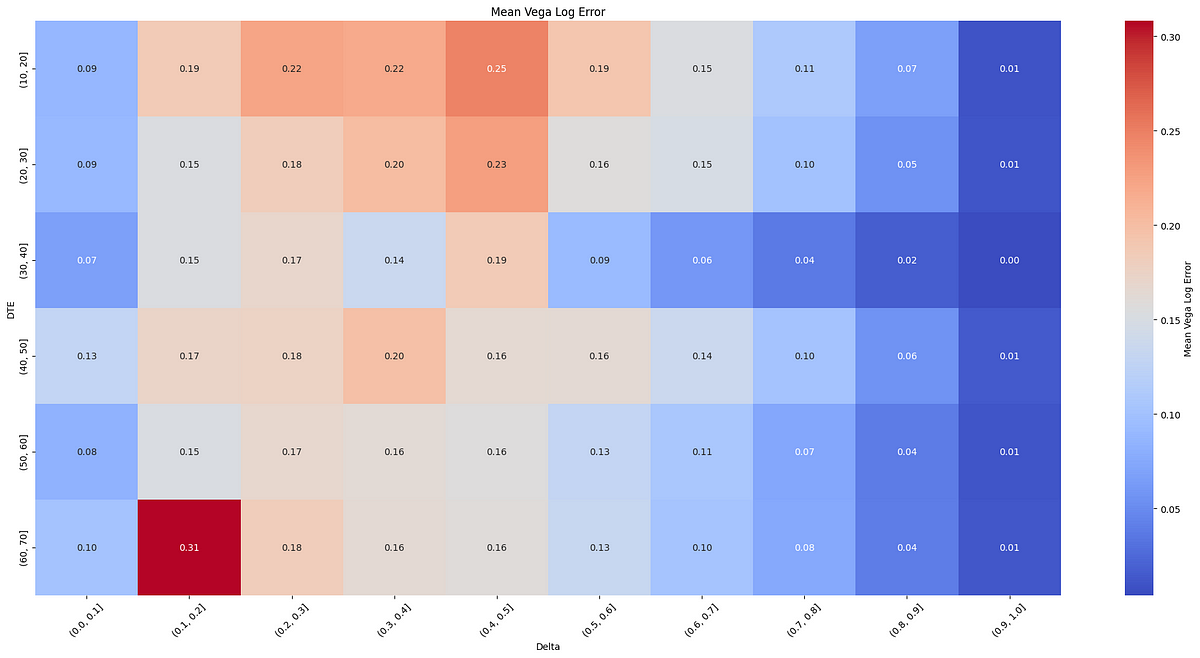
\includegraphics[width=0.85\textwidth]{heston_vega_heatmap.png}
  \caption{Vega-Sensitivität unter dem Heston-Modell für verschiedene Strikes und Laufzeiten.}
\end{figure}


\subsection*{8. Preisberechnungsmethoden im Vergleich}
\begin{tcolorbox}[title=Wann welche Methode?]
\begin{itemize}
  \item \textbf{Fourier-Methoden (z.\,B. Carr-Madan):} Sehr effizient für europäische Optionen, wenn charakteristische Funktion bekannt.
  \item \textbf{Monte Carlo:} Flexibel bei exotischen Optionen oder Pfadabhängigkeiten (z.\,B. Asian, Barrier), aber langsamer.
  \item \textbf{Finites Differenzenverfahren:} Für PIDE (z.\,B. bei Heston mit Jumps), gut für Preisoberflächen.
\end{itemize}
\end{tcolorbox}

\subsection*{9. Modellhierarchie in der Volatilitätsmodellierung}
\begin{tcolorbox}[title=Vergleich der Modelle]
\begin{itemize}
  \item \textbf{Black-Scholes:} Konstante Volatilität → keine Smile-Effekte.
  \item \textbf{Heston:} Stochastische Volatilität → Smile, Mean-Reversion.
  \item \textbf{Bates:} Heston + Sprungprozess → besser bei Earnings-/Crash-Risiken.
  \item \textbf{SABR:} Besonders für Zinsderivate mit starkem Skew.
\end{itemize}
\end{tcolorbox}

\subsection*{10. Typische Anwendungen in der Praxis}
\begin{tcolorbox}[title=Einsatzbereiche des Heston-Modells]
\begin{itemize}
  \item Pricing von \textbf{exotischen Optionen} mit Volatilitätskomponenten (z.\,B. Barrier, Cliquet).
  \item \textbf{Volatility Surface Calibration} im Derivatehandel.
  \item \textbf{XVA-Analysen}: Adjustments für Credit, Funding oder Capital.
  \item \textbf{Stresstests}: Reaktion auf Schocks bei IV-Surfaces.
\end{itemize}
\end{tcolorbox}

\end{document}